% MplTplt - Yet another LaTeX template for Modern Physics Lab, PKU.
% Copyright (C) 2014 Huang Kangjing and contributors

% This work is completely rewritten basing on the work of Cao Chuanwu
% and Sun Sibai, with texts in the template originally coming from the
% Modren Phys. Lab.

% This file is released under the MIT license.
%
% Permission is hereby granted, free of charge, to any person obtaining a copy
% of this software and associated documentation files (the "Software"), to deal
% in the Software without restriction, including without limitation the rights
% to use, copy, modify, merge, publish, distribute, sublicense, and/or sell
% copies of the Software, and to permit persons to whom the Software is
% furnished to do so, subject to the following conditions:
% 
% The above copyright notice and this permission notice shall be included in
% all copies or substantial portions of the Software.
% 
% THE SOFTWARE IS PROVIDED "AS IS", WITHOUT WARRANTY OF ANY KIND, EXPRESS OR
% IMPLIED, INCLUDING BUT NOT LIMITED TO THE WARRANTIES OF MERCHANTABILITY,
% FITNESS FOR A PARTICULAR PURPOSE AND NONINFRINGEMENT. IN NO EVENT SHALL THE
% AUTHORS OR COPYRIGHT HOLDERS BE LIABLE FOR ANY CLAIM, DAMAGES OR OTHER
% LIABILITY, WHETHER IN AN ACTION OF CONTRACT, TORT OR OTHERWISE, ARISING FROM,
% OUT OF OR IN CONNECTION WITH THE SOFTWARE OR THE USE OR OTHER DEALINGS IN
% THE SOFTWARE.
%

% This template depends on the "revtex4.1" package from APS Journals
% <http://publish.aps.org/revtex/revtex-faq>, and the Chinese handling
% is done with XeLaTeX engine and package "xeCJK". Please ensure these
% packages are available in your chosen Tex software distribution.

% Document created using this template should be compiled with XeLaTeX
% engines rather than plain LaTeX or plain TeX engines.

% The non-ASCII texts of this template is encoded in UTF-8 encoding.
% Please note that XeLaTeX only accepts UTF-8 encoded documents, so
% set your editor to use UTF-8 while creating documents with this template.

% Recommended TeX software distribution to use with this template is
% Tex Live developed by the TeX User Group (TUG), please visit the home
% page of the distribution <https://www.tug.org/texlive/> for further details.

% NOTE THAT IMPORTANT INSTRUCTIONS HAS BEEN WRITTEN AS UPPERCASE COMMENTS
% IN THE TEXT, PLEASE READ THEM CAREFULLY AND FOLLOW THEM TO MAKE THE
% TEMPLATE WORK!

% Any further contributions to the template is welcome, please send
% pull requests through github or send mail to maintainer.

% For any other questions, please do not hesitate to contact maintainer.

% Current maintainer:
% Huang Kangjing <huangkangjing@gmail.com>

% Contributors:
% Sun Sibai <niasw@pku.edu.cn>
% Cao Chuanwu <>
% Huang Kangjing <huangkangjing@gmail.com>


\documentclass[aps,pre,12pt,preprint,onecolumn,showpacs,showkeys]{revtex4-1}

% Setting up Chinese handling.
\usepackage{fontspec,xeCJK}

% Setting up fonts.
% PLEASE MODIFY ALL THESE FONT NAMES ACCORDING TO YOUR FONT
% INSTALLATION AND PERFERENCE.

% Setting up main fonts and mono fonts.
\setmainfont{Liberation Serif}
\setmonofont{Liberation Mono}
% SimSun is required font for the main body of the text.
\setCJKmainfont[AutoFakeBold=5,AutoFakeSlant]{SimSun}
\setCJKmonofont[AutoFakeBold=2,AutoFakeSlant]{SimHei}

% Setting up alternative font families.
% Note that these three fonts below are required fonts in document
% title, section headings and figure captions.
\newCJKfontfamily\heiti[AutoFakeBold=2,AutoFakeSlant]{SimHei}
\newCJKfontfamily\fangsong[AutoFakeBold=5,AutoFakeSlant]{FangSong}
\newCJKfontfamily\kaiti[AutoFakeBold=5,AutoFakeSlant]{KaiTi}

% Setting up paragraph indent.
\parindent 2em

% Setting up macros for Chinese-style font size setting.
\newcommand{\fseight}{\fontsize{5.02}{6.02}\selectfont}
\newcommand{\fsseven}{\fontsize{5.52}{6.62}\selectfont}
\newcommand{\fsssix}{\fontsize{6.52}{7.83}\selectfont}
\newcommand{\fssix}{\fontsize{7.53}{9.03}\selectfont}
\newcommand{\fssfive}{\fontsize{9.03}{10.84}\selectfont}
\newcommand{\fsfive}{\fontsize{10.54}{12.65}\selectfont}
\newcommand{\fssfour}{\fontsize{12.05}{14.45}\selectfont}
\newcommand{\fsfour}{\fontsize{14.05}{16.86}\selectfont}
\newcommand{\fssthree}{\fontsize{15.06}{18.07}\selectfont}
\newcommand{\fsthree}{\fontsize{16.06}{19.27}\selectfont}
\newcommand{\fsstwo}{\fontsize{18.07}{21.68}\selectfont}
\newcommand{\fstwo}{\fontsize{22.08}{26.50}\selectfont}
\newcommand{\fssone}{\fontsize{24.09}{28.91}\selectfont}
\newcommand{\fsone}{\fontsize{26.10}{31.32}\selectfont}
\newcommand{\fsszero}{\fontsize{36.14}{43.36}\selectfont}
\newcommand{\fszero}{\fontsize{42.16}{50.59}\selectfont}

% Replace words to Chinese corespondence.
\renewcommand\appendixname{附录}
\renewcommand\abstractname{}
\renewcommand\tablename{表}
\renewcommand\figurename{图}

% Replace words in revtex4-1 to Chinese corespondence.
\makeatletter
\def\@pacs@name{\heiti\fssfour \textbf{PACS码:}\normalfont}
\def\@keys@name{\heiti\fssfour \textbf{关键词:}\normalfont}
\def\Dated@name{日期:}
\def\Received@name{\fssfive 接收 }
\def\Revised@name{\fssfive 修订 }
\def\Accepted@name{\fssfive 采纳 }
\def\Published@name{\fssfive 发表 }
\makeatother

% Change label style of enumerate.
\renewcommand{\labelenumi}{\alph{enumi}.}

% Setting up geometry.
\usepackage{geometry}
\geometry{top=2.54cm,bottom=2.54cm,left=3cm,right=3cm}

% Setting up line space.
\usepackage{setspace}
\linespread{1.6}

% Setting up hyperreferences.
\usepackage{hyperref}
\hypersetup{colorlinks=true}

% Setting up styles for section headings.
\usepackage{titlesec}
\titleformat*{\section}{\bf\fangsong\fsfour}
\titleformat*{\subsection}{\bf\fangsong}

% Loading packages for image handling.
\usepackage{subfig}
\usepackage{graphicx,psfrag,epsfig}

% Setting up caption styles.
\usepackage{caption}
\DeclareCaptionFont{kaiti}{\kaiti}
\DeclareCaptionFont{bfheiti}{\bf\heiti}
\captionsetup{font=small,format=plain,labelfont=bfheiti,%
  textfont=kaiti,justification=raggedright,%
  singlelinecheck=false}

% Loading packages for math typings.
\usepackage{amsmath,amsfonts,amssymb,amsthm,bm,upgreek}
\usepackage[mathscr]{eucal}
\usepackage[separate-uncertainty=true]{siunitx}


\begin{document}

% Title and author info.
\title{\bf\heiti\fsthree 核磁共振\vspace{15mm}}
\author{\fangsong\fsfour 黄康靖\vspace{2mm}}
\affiliation{\normalfont\fssfour 北京大学物理学院2014级本科生~~~~学号{masked student id}\vspace{2mm}}
\date{\today}
\keywords{核磁共振,g因子,磁场测量}
\email{ huangkangjing@gmail.com; {masked phone number}}

% Abstract.
\begin{abstract}
  \vspace{10mm}
  \begin{spacing}{1.5}
    \fssfour
磁矩不为零的微观粒子的磁矩是量子化的,当它们处在外磁场中时空间取向和能量
也是量子化的,造成能级的塞曼分裂.此时在垂直于磁场方向加一合适的射频
场,将会出现磁共振现象.原子核的磁共振现象和相关的实验技术是重要的物理现
象和实验技术,在许多领域有广泛的应用,且可用于原子核磁矩的精确测量.
本实验利用核磁共振原理和相关技术,完成了磁场的校准和氟核$g$因子的测量.
  \end{spacing}
\end{abstract}

% The main body of the document goes from here.
\maketitle
\fssfour
\section{引言}

Pauli在1924年研究某些元素光谱的精细结构时首先提出了核磁矩与核自旋的概
念,但在当时由于光学仪器分辨本领的限制,妨碍了对核磁矩的精确测量.1939
年I.Rabbi在真空中的氢分子束实验中首次观察到核磁共振现象,并利用核磁共振方法,实
现了对核磁矩更为精确的测量.

磁共振是重要的物理现象.磁矩不为零的微观粒子(包括电子、质子、中子、原子
核、原子、离子等)其磁矩是量子化的.当粒子处于外磁场中时其空间取向也是量
子化的,空间取向量子化的磁矩在外磁场中的能量也是量子化的,造成能级的塞曼
分裂.此时若在垂直于磁场方向施加一个频率合适的交变电磁场,将导致粒子在
相邻的塞曼能级之间跃迁,这就是磁共振.利用磁共振现象可以用来研究粒子的结
构与性质.

近代磁共振技术在1946年由美国Harvard大学的Purcell和Pound以及Stanford大
学的Bloch和Hanson同时独立设计.这些技术所需要的设备和实验方法都比较简单,
但却提高了核磁矩的测量精度.\cite{book}

本实验利用稳态核磁共振的原理和实验方法,进行了磁场的校准以及氟核
和氘核的$g$因子测量.

\section{背景}

\subsection{原子核的磁矩}

角动量$\bm{P}$不为零的原子核具有与角动量共线取向的磁矩$\bm{\mu}$,即
\begin{equation}
\bm{\mu} = \gamma\bm{P}  
\end{equation}
其中$\gamma$称为原子核的旋磁比,可以用实验方法测出.

这一关系也通常写成
\begin{equation}
\bm{\mu} = g\cdot\frac{q}{2m_N}\bm{P}
\end{equation}
其中$q$是原子核电荷,$m_N$是核的质量,$g$是一个无量纲的因子,即我们通常所
说的$g$因子.

另一方面,若对于质子来讲,对应于玻尔磁子可以引入核磁子
\begin{equation}
\mu_N = \frac{eh}{2m_p}
\end{equation}
我们把核磁子作为核磁矩的计量单位,同时把$\hbar$作为角动量的计量单位,那
么,我们可以定义$g$因子为
\begin{equation}
g = \frac{\bm{\mu}/\mu_N}{\bm{P}/\hbar} =
\frac{\gamma/2\pi}{\mu_N/h}
\end{equation}
式中$\mu_N/h$是一个常量,从而在表征原子核磁矩方面,$g$和$\gamma$是等效的.

\subsection{核磁共振的量子力学描述}

根据量子力学的相关原理,微观粒子(包括原子核)的角动量和磁矩是量子化的,并
且这一量子化应当使用自旋量子数$I$表征,他们的数值满足:
\begin{equation}
\begin{cases} P = \sqrt{I(I + 1)}\hbar \\
\mu = g \sqrt{I(I+1)}\mu_N \end{cases}, I = 0,\frac{1}{2},1,
\frac{3}{2} \dots
\end{equation}

另一方面,微观粒子的角动量在空间的取向也应当是量子化的,称为空间量子化.一
个自旋量子数为$I$的微观粒子,它的角动量和磁矩在外磁场方向的投影只能取如
下的数据:
\begin{equation}
\begin{cases}P_z = m\hbar \\ 
\mu_z = \gamma m \hbar\end{cases}, m = I, I-1, \dots, -I+1, -I
\end{equation}


既然磁矩的取向是空间量子化的,那么,磁矩与外磁场的相互作用能也是不连续的,形
成分立的能级
\begin{equation}
E = - \bm{\mu} \cdot \bm{B} = -\mu_zB = -m\gamma\hbar B , m = I,
\dots, -I
\end{equation}
这一现象称为塞曼分裂,两个相邻的塞曼能级间的能量差为
\begin{equation}
\Delta E = \gamma \hbar B
\end{equation}

当垂直于恒定磁场$B$的平面上同时存在一个射频场,并且其频率满足一定条件时,会
发生磁偶极共振跃迁.磁偶极共振跃迁的选择定则是$\Delta m = \pm 1$,由此可
以得到共振时的频率条件
\begin{equation}
\omega = \gamma B \text{~~~或~~~} \nu=\frac{\gamma}{2\pi}B
\end{equation}

容易得到,在磁共振中,由于塞曼能级之间的间距非常小,自发辐射完全可以忽略,
因此当下能级粒子数比上能级粒子数多时,发生共振吸收时系统吸收射频场能量,
当上下能级粒子数相等时,虽然有共振跃迁但是观察不到能量吸收.

根据波尔茨曼分布,上下能级的粒子数满足
\begin{equation}
\frac{N_{20}}{N_{10}} = \exp (-\Delta E/kT)
\end{equation}
其中$N_{20},N_{10}$分别是上下能级的粒子数,一般情形下,我们有$\Delta E
\ll kT$,从而下能级与上能级的粒子数之差为
\begin{equation}
n_0 \approx \frac{\gamma\hbar B}{2kT}N
\end{equation}
$N$为粒子总数.

这一差数的存在使得观察核磁共振吸收成为可能.


\subsection{核磁共振的宏观理论}

在矢量模型的基础上,用经典的方法处理可以得到核磁共振的宏观理论.

从经典物理图像来讲,核磁共振是自旋不为零的粒子在外磁场中的拉莫尔进动行
为.并且,整个系统宏观上的可观测量应当是单位体积中微观磁矩矢量的总和,即
磁化强度矢量
\begin{equation}
\bm{M} = \sum_i\bm{\mu_i}
\end{equation}


于是,可以得到磁化强度矢量在拉莫尔进动效应下的动力学方程:
\begin{equation}
\frac{d\bm{M}}{dt} = \gamma\bm{M} \times \bm{B}
\end{equation}

另一方面,实际材料在热平衡状态下,磁化强度矢量应当有相应的热
平衡值$\bm{M}_0$;并且当磁化强度矢量偏离热平衡数值之后,会有自发的物理过
程,使得磁化强度矢量趋向于热平衡数值,即所谓的弛豫过程.可以得到,弛豫过程
的动力学满足以下规律:
\begin{equation}
\begin{cases}
\frac{dM_z}{dt} = - \frac{1}{T_1}(M_z - M_0) \\
\frac{dM_x}{dt} = - \frac{1}{T_2}M_x \\
\frac{dM_y}{dt} = - \frac{1}{T_2}M_y
\end{cases}
\end{equation}
其中$T_1$称为纵向弛豫时间,$T_2$称为横向弛豫时间,$M_0$为热平衡态下$z$方
向的磁化强度矢量值,满足
\begin{equation}
M_0 = \frac{I+1}{3I}\frac{N\mu^2}{kT}B_0
\end{equation}

从而,可以写出同时考虑磁场作用与弛豫效应的影响的整个系统的动力学方程
\begin{equation}
\frac{d\bm{M}}{dt} = \gamma\bm{M}\times\bm{B} -
\frac{1}{T_2}(M_x\bm{i} + M_y\bm{j}) - \frac{1}{T_1}(M_z -
M_0)\bm{k}
\end{equation}
称为布洛赫方程式.

在核磁共振实验中,除了外加的恒定磁场以外,还会在与恒定磁场相垂直的平面上
加上一个线偏振射频场,这个射频场可以看做是左旋圆偏振场与右旋圆偏振场的
叠加.在这两个场中,只有与磁化强度矢量做拉莫尔进动方向一致的射频场才会起
作用.

在伴随有效圆偏振射频场一起旋转的坐标系中解布洛赫方程式,便可以得到方程
的稳态解:
\begin{equation}
\begin{cases}
u = \frac{\gamma B_1 T^2_2(\omega_0 - \omega)M_0}{1 + T_2^2(\omega_0 -
  \omega)^2 + \gamma^2B_1^2T_1T_2}\\
v= \frac{-\gamma B_1 M_0T_2}{1 + T_2^2(\omega_0 -
  \omega)^2 + \gamma^2B_1^2T_1T_2} \\
M_z = \frac{\left[1 +T^2_2(\omega_0 - \omega) \right]M_0}{1 + T_2^2(\omega_0 -
  \omega)^2 + \gamma^2B_1^2T_1T_2}
\end{cases}
\end{equation}
其中$u$为$xoy$平面上磁化强度矢量与射频场磁场方向一致的矢量分量,相当于
动态复数磁导率的实部,称为色散信号;$v$为$xoy$平面上磁化强度矢量与射频
场磁场方向垂直的矢量分量,相当于动态复数磁导率的虚部,称为吸收信号.在实
验中,通过测量电路的不同处理方式,可以观察到色散信号或者吸收信号.

最后,通过对于吸收信号的形式分析,我们可以得到吸收谱线的半峰宽(FWHM:Full Width at Half Maxumum)为
\begin{equation}
\Delta \omega = \frac{2}{T_2}
\end{equation}
于是,通过测量吸收谱线的半宽度,我们可以测量材料的磁化强度矢量的横向弛豫
时间.

\section{实验}

实验装置的示意图如图~\ref{fig:ins}

\begin{figure}[htbp]
  \centering
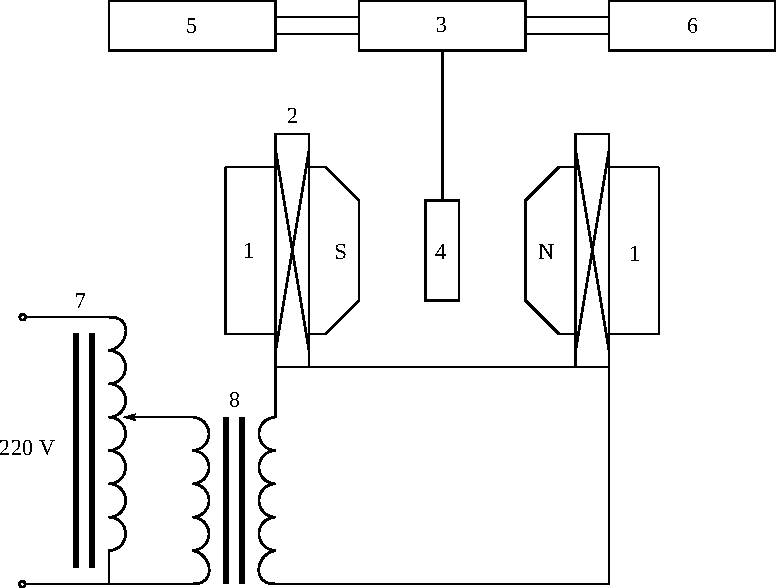
\includegraphics[width=.7\textwidth]{drawing.pdf}
\caption{\label{fig:ins}%
实验装置的方框图,图中各项为:1.永久磁铁~~2.扫场线圈~~3.电路盒~~4.样品和
振荡线圈~~5.数字频率计~~6.示波器~~7.可调变压器~~8.220V/6V变压器
}
\end{figure}

\subsection{固定磁场}

本实验的固定磁场由永久磁铁提供$B_0 > \SI{0.5}{T}$,在均匀区
$(\SI{5}{mm})^2$范围内均匀性优于$\num{1e-5}$,可以满足核磁共振实验的相
应要求.

\subsection{射频磁场}

射频磁场由电路盒中的振荡电路通过振荡线圈产生,产生的磁场是线偏振的射频
磁场.如前文所述,该线偏振射频场可以看作两个旋转方向相反的圆偏振磁场的叠
加,而其中的有效射频场只有一个.

\subsection{接收电路}

我们采用单线圈法,振荡线圈既是发射线圈,也是接收线圈.电路盒中采用边限振
荡器作为测量电路.边限振荡器在调节适当的情况下,不会工作在稳定
状态,而是工作在刚刚起振的边缘状态,此时任何电路参数的改变都会引起工作状
态变化.当共振发生时样品要吸收射频场能量,使得振荡线圈$Q$值减小,导致振荡
器工作状态改变,表现在振荡波形包络线发生变化,该信号经检波、放大处理
后,从电路盒背面的"检波"端口输出,在示波器上即可观察到共振吸收信号.

\subsection{扫~场}

实验采用扫场的方式观察核磁共振吸收信号,即通过改变磁场$B_0$的大小,来改
变$\omega_0$的值,从而改变$\omega-\omega_0$这一相对值的大小,进而实现对
于核磁共振吸收信号的观测.


\section{实验结果及分析讨论}

实验的所有直接测量结果见表~\ref{tab:rawdata}.

\begin{table}[t]
\caption{\label{tab:rawdata}%
实验的直接测量数据表.表中的共振频率为在示波器上观察到明确核磁共振吸收
信号的对应频率;上限共振识别频率与下限共振识别频率为调节射频场频率时,刚
好使得共振信号不可识别的最大和最小频率,用于计算测量的误差.}
\begin{ruledtabular}
\begin{tabular}{llll}
样品 & 共振频率 $f$/MHz & 上限共振识别频率  $f_{U}$/MHz & 下限共振识别
频率 $f_{D}$/MHz \\ \hline
水 & 21.0706 & 21.0745 & 21.0666 \\
聚四氟乙烯 & 19.8206 & 19.8432 & 19.7930
\end{tabular}\end{ruledtabular}
\end{table}

实验首先通过测量"水"样本中的质子共振信号,为装置中的永久磁铁磁场定标,取
质子的回旋频率为\cite{book}
\begin{equation}
\frac{\gamma}{2\pi} = \SI{42.5763888 \pm
  0.0000018}{MHz/T}
\end{equation}
计算得到永久磁铁磁场的测量值应为
\begin{equation}
B = \SI{0.494889 \pm 0.000002}{T}
\end{equation}

实验接下来通过测量"聚四氟乙烯"样本中的原子核共振信号,测量了氟原子核的
$g$因子.取玻尔磁子为\cite{book}
\begin{equation}
\frac{\mu_N}{h} = \SI{7.62259396 \pm 0.00000031}{MHz/T}
\end{equation}
计算得到氟原子核的$g$因子测量值应为
\begin{equation}
g = \num{5.25419 \pm 0.00009}
\end{equation}

实验还观察了"纯水"样本的特征和"氟化氢"样本的特征.

"纯水"样本的共振峰和"水"样本的共振峰一致,但是信号强度要弱的多.

"氟化氢"样本存在两个共振峰,分别与"水"样本的共振峰位置和"聚四氟乙烯"样
本的共振峰位置一致.

实验最后估测了"聚四氟乙烯"样品的横向弛豫时间,测得这一样品的共振峰半峰宽(FWHM)
为\begin{equation}
\Delta\omega = \SI{3.267e4}{s^{-1}}
\end{equation}
计算得到估测的横向弛豫时间.
\begin{equation}
T_2 \approx \SI{6.12e-5}{s}
\end{equation}

\section{致谢}

感谢邹宇斌老师在实验中认真而专业的指导.


% Bibliography example.
\begin{thebibliography}{}
\bibitem{book} 吴思成,王祖铨~2010 近代物理实验(第三版)(北京:高等教
育出版社)第306页. 
\bibitem{report} 黄康靖~北京大学2014年近代物理实验报告:用$\beta$粒子
  检验相对论的动量-动能关系.
\end{thebibliography}

\clearpage
\appendix
\section{思考题}
\begin{enumerate}
\item  这是因为"纯水"样品中未掺入三氯化铁,于是纵向弛豫时间较短,导致饱
  和因子较大,从而导致了信号过于小.
\item 这是因为"氢氟酸"样品中同时含有氢原子核和氟原子核,所以可以看到两
  个峰
\end{enumerate}


\end{document}
